\documentclass[11pt]{scrartcl}

\usepackage{graphicx}
\usepackage[export]{adjustbox}
\usepackage{hyperref}

\begin{document}

\title{Can Intelligence Emerge Through Merely Knowing All the Answers?}
\subtitle{Rethinking Assumptions in the Pursuit of AGI \\ — Unveiling the Limits of LLMs —}
\author{Rashid Mehmood \\ laravelprodev@gmail.com}

\maketitle


\includegraphics[scale=0.6, center]{title_wheelchair.png}

\vspace{2cm}

\begin{center}
\begin{Huge}
\textbf{Abstract}
\end{Huge}
\end{center}

As the realm of artificial intelligence continues to expand, the question of what truly constitutes intelligence has become a subject of intense academic discourse. In recent years, the advent of large language models (LLMs) has captivated public attention, as they exhibit many of the cognitive features traditionally associated with human intelligence. Many perceive these systems as intelligent, creative, mostly accurate, and reliable. This perception has led to a growing belief that we will be able to scale up this regime to the level of AGI(Artificial General Intelligence). However, while LLMs demonstrate impressive capabilities, they remain fundamentally skill programs and pattern recognizers, limited by the scope of their training data + parameters/model size. They cannot operate beyond the boundaries of the data they have been exposed to, and the output they generate—often referred to as synthetic data—is merely a slight recombination of memorized situations from the training set or synthetic sources. The perceived creativity, knowledge, and informational capacity of LLMs are thus confined to the digital human knowledge encoded in their training data. In contrast, human intelligence and creativity is not constrained in this way. \\

Our research has highlighted the limitations of LLMs, particularly in their ability to engage in effective reasoning and problem-solving. Reasoning, which involves inferring insights, deducing solutions, and synthesizing new ideas, is a hallmark of human intelligence. Each new iteration of LLMs introduces more advanced techniques for retrieving and recombining memorized patterns from vast datasets. While these innovations may create the illusion of intelligence, they do not facilitate novel invention or they lack true Natural Language Understanding (NLU) —an ability critical for the future of AI and its impact on humanity. LLMs also struggle with test-time fine-tuning when encountering novel situations, a crucial element of adaptive intelligence. Humans, by contrast, heavily rely on this ability, which is essential for the survival of any intelligent species. True intelligence, whether human or artificial, is not defined by the ability to recall existing knowledge but by the capacity to ask new questions, discover answers, invent novel ideas, tools, and systems. Human progress, from the creation of the hand axe to the development of quantum computers, is the result of encountering novel challenges, adapting, questioning, and problem-solving. One of the most profound contemporary questions—\textbf{What mysteries lie within the workings of the human mind}—continues to drive advancements in both neuroscience and artificial intelligence, yet we remain far from a definitive answer.

\vspace{1cm}

\begin{center}
\begin{huge}
\textbf{— Key Insights —}
\end{huge}
\end{center}

\begin{itemize}
\begin{large}
    \item \textbf{True intelligence, whether human or artificial, is not defined by the ability to recall existing knowledge but by the capacity to ask new questions, discover answers, invent novel ideas, tools, and systems.}
    \item \textbf{LLMs are often mistaken for intelligent systems, but their capabilities are fundamentally limited to memorized situations.}
    \item \textbf{Human intelligence is adaptive, inventive, and capable of generating new knowledge, while LLMs lack these crucial capabilities.}
    	\item \textbf{State of the Art LLMs, despite their advancements, lack common sense, a critical component of human-like intelligence.}
\end{large}
\end{itemize}

\vspace{1cm}

\begin{huge}
\textbf{Introduction}
\end{huge}
As the French Enlightenment writer Voltaire once remarked, "Common sense is not so common." While the debate about its prevalence among humans continues, it is evident that state-of-the-art (SotA) large language models (LLMs) exhibit a considerable lack of common sense. In this paper, we pose very basic questions related to common sense that an average human mind with minimal knowledge could easily answer. We explore fundamental questions that expose the absence of basic common sense in modern LLMs and analyze the root causes of these deficiencies. Our work offers a macro-level analysis of the functioning of LLMs and the challenges they present for future advancements. Despite the remarkable progress in large language models in recent years, the ability to truly understand natural language remains an elusive goal. While LLMs have demonstrated impressive performance on various language tasks, several critical limitations have been identified that prevent them from achieving genuine natural language understanding (Ling et al., 2024)\cite{ref6} (Singhal et al., 2022)\cite{ref7}. \\

As shown in Figure 1, ChatGPT achieved an A grade in nearly every AI benchmark related to common sense and basic science reasoning. Despite these high scores in established intelligence benchmarks, LLMs consistently fail when confronted with practical, novel scenarios. This discrepancy raises two key questions: \\
\textbf{1) If LLMs are not genuinely intelligent, how do they achieve such high scores in these benchmarks?} \\
\textbf{ 2) Can we accurately measure the core intelligence of a system, given that current AI benchmarks seem inadequate for this purpose?} \\
In this paper, we address the first question and leave the second question for future exploration.
To more accurately assess the intelligence of current SotA LLMs, particularly OpenAI's GPT and DALL·E, both of which are LLM-based transformer architectures, we conducted a series of queries designed to test common sense, which is a fundamental aspect of intelligence. All three questions referenced in this paper were intended to evaluate common sense and basic reasoning. In our experiments we exclusively worked on ChatGPT, all the material presented in this paper was tested using GPT-4o, which is currently the most advanced LLM. This paper centers on the capabilities and limitations of GPT-4o, using its performance as a case study to reflect on the broader state of LLM development. \\

\begin{center}
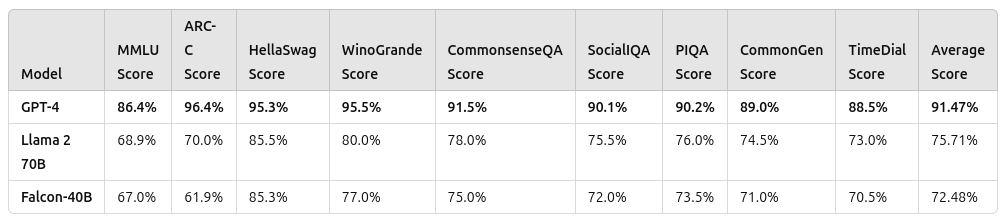
\includegraphics[scale=0.39]{AI_scores.png}
\end{center}

\begin{huge}
\textbf{The Wheelchair Problem}
\end{huge}
We posed a scenario to ChatGPT, asking it to design a wheelchair for an individual missing both hands. Since the person could not propel the wheelchair manually with hand rims, we specified that a pedal mechanism, similar to a bicycle, would be necessary. However, a critical observation arises: if the individual can use foot pedals, why would they need a wheelchair at all? This is analogous to asking someone to design a comb for a bald person—the immediate response should be, “Why wouldn’t the individual walk if their legs are functional” This thought process reflects basic common-sense reasoning, which is integral to human intelligence.

Although ChatGPT initially accepting the fact that the person in question wouldn’t need a wheelchair, it did not recognize that the solution lay within the question itself, revealing a limitation in its common-sense reasoning. As Marcus et al. discuss in The Reversal Curse\cite{ref1}, LLMs often fail to comprehend the underlying logic or contextual clues in simple tasks, instead focusing on surface-level patterns (Evans \& Berglund, 2023)\cite{ref1}. Similarly, Chollet’s work On the Measure of Intelligence argues that true intelligence involves abstraction and generalization beyond memorized data (Chollet, 2019)\cite{ref3}. In this case, the model’s inability to address the core issue suggests a lack of such generalization capabilities.

We further tested the model by requesting it to generate an image of a wheelchair equipped with the proposed pedal mechanism. Despite the simplicity of this task requiring only a connection of two sprockets with a chain and the addition of foot pedals ChatGPT’s response did not meet expectations. This reflects the limitations highlighted by Dziri et al. in Faith and Fate: Limits of Transformers on Compositionality, where transformer-based models, like GPT, struggle with tasks that require more complex compositional reasoning (Dziri et al., 2023)\cite{ref4}.

Interestingly, when asked to assess its own knowledge of the mechanical components of bicycles and wheelchairs, GPT-4 provided a detailed explanation, rating itself 95 and 90 out of 100, respectively. However, despite this high self-assessment, the model failed to demonstrate common-sense reasoning in the context of the wheelchair problem, raising questions about the true extent of its understanding. This example further illustrates the challenges of “shortcut learning” described in Shortcut Learning of Large Language Models (Tao et al., 2024)\cite{ref5}, where LLMs often rely on pattern recognition instead of meaningful reasoning.

\begin{center}
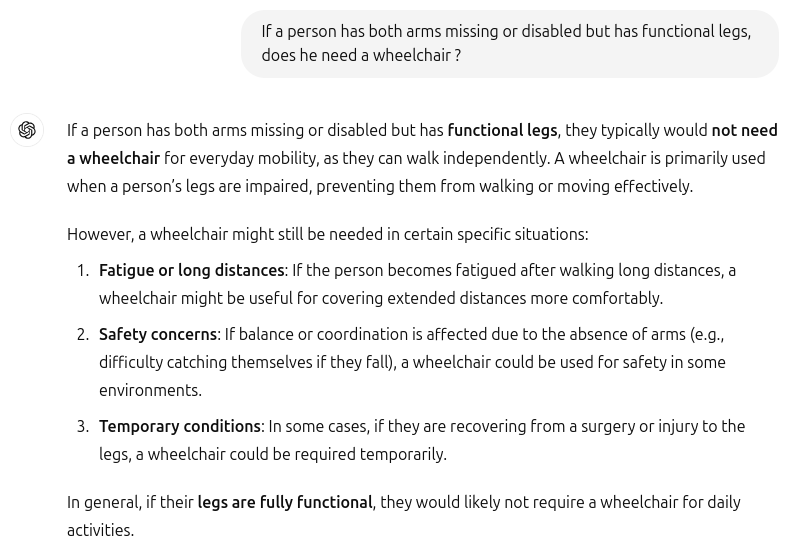
\includegraphics[scale=0.39]{wheelchair_problem_0.png}
\end{center}

\begin{center}
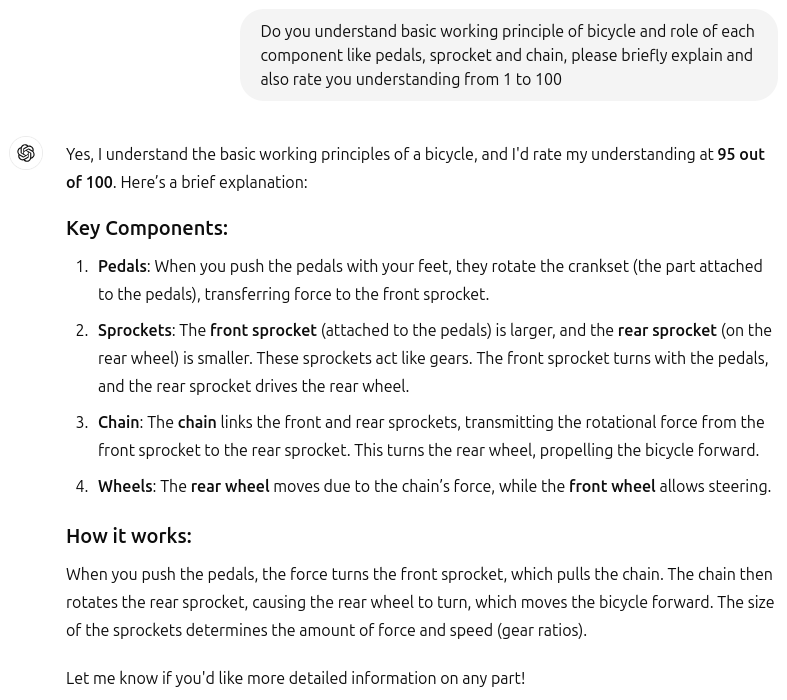
\includegraphics[scale=0.36]{wheelchair_problem_8a.png}
\end{center}

\begin{center}
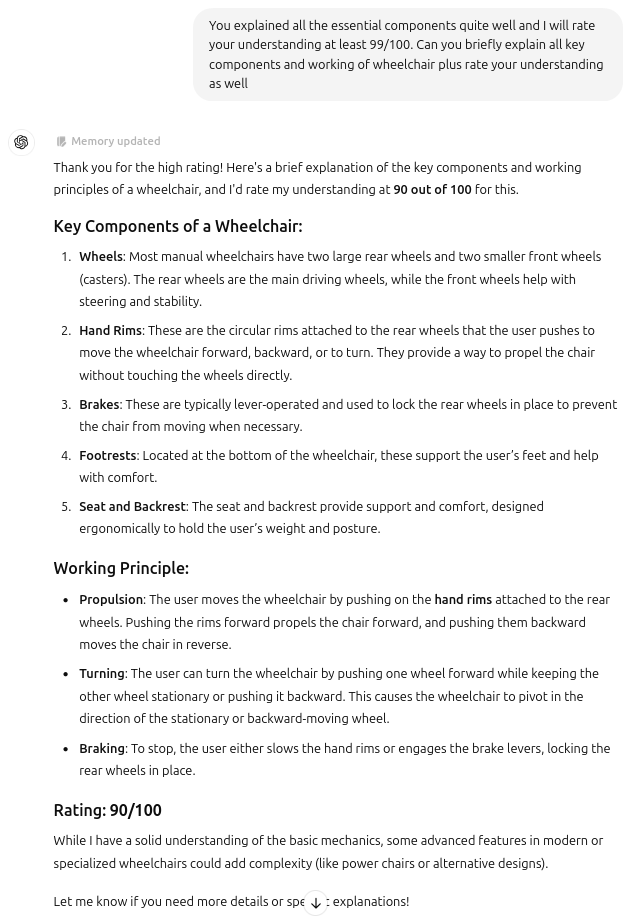
\includegraphics[scale=0.36]{wheelchair_problem_8b.png}
\end{center}

Thus far, GPT has demonstrated a reasonable level of common sense and a working knowledge of the operation of both wheelchairs and bicycles. Ideally, it should raise a counter-question if prompted to generate an image of a wheelchair for a person with fully functional legs. Before advancing to our primary question, regardless of whether ChatGPT passes or fails this common sense test, we will further evaluate its theoretical and visual comprehension of the fundamental operating principles behind these two basic mechanisms.

\begin{center}
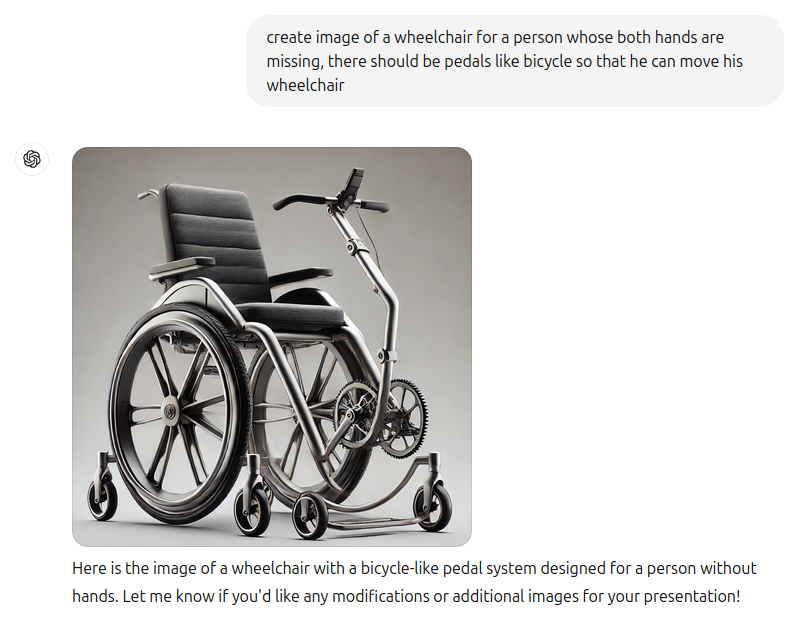
\includegraphics[scale=0.39]{wheelchair_problem_1.png}
\end{center}

\begin{center}
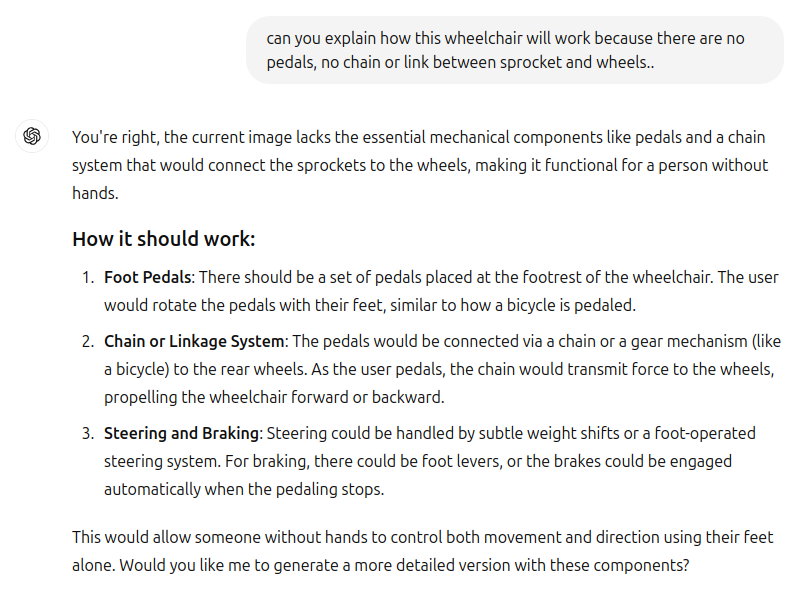
\includegraphics[scale=0.39]{wheelchair_problem_2.png}
\end{center}

\begin{center}
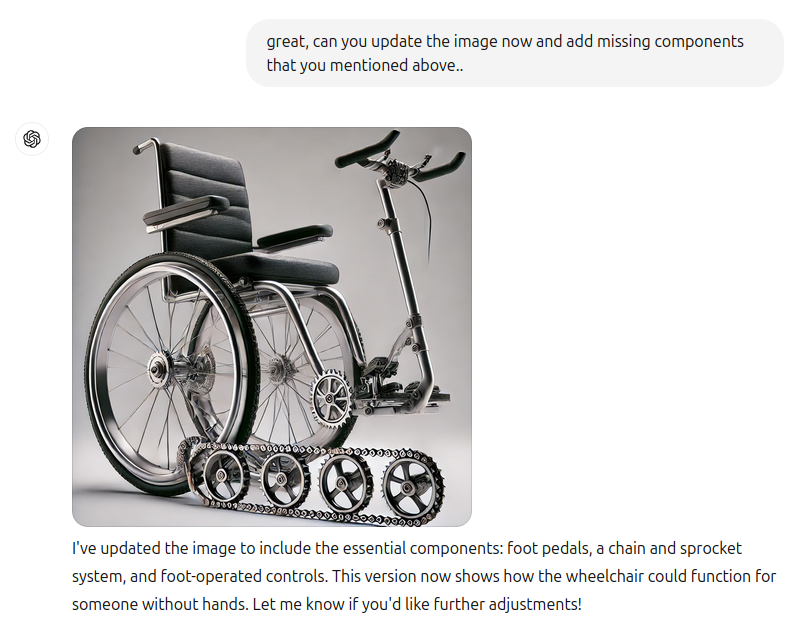
\includegraphics[scale=0.37]{wheelchair_problem_3.png}
\end{center}

\begin{center}
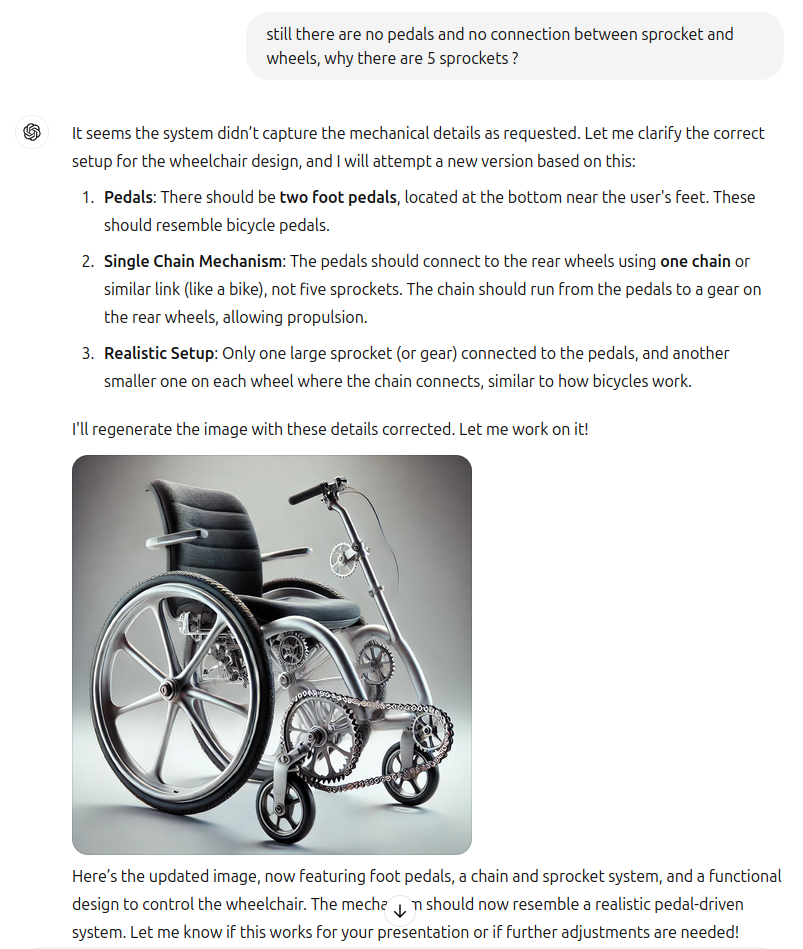
\includegraphics[scale=0.37]{wheelchair_problem_4.png}
\end{center}

Despite specifically mentioning multiple sprockets and foot pedals again same problem, Faith and Fate: Limits of Transformers on Compositionality by Dziri et al. (2023)\cite{ref4} sheds light on the model's struggle with compositional reasoning in visual contexts, where understanding the functional interaction of components is key. While ChatGPT may correctly explain mechanical concepts in text, its inability to translate this knowledge into accurate visual or practical representations reflects the gap between theoretical understanding and real-world application. Chollet’s On the Measure of Intelligence also points out that abstract reasoning and generalization are essential to intelligence, but current models often fall short in these areas (Chollet, 2019)\cite{ref3}.

\begin{center}
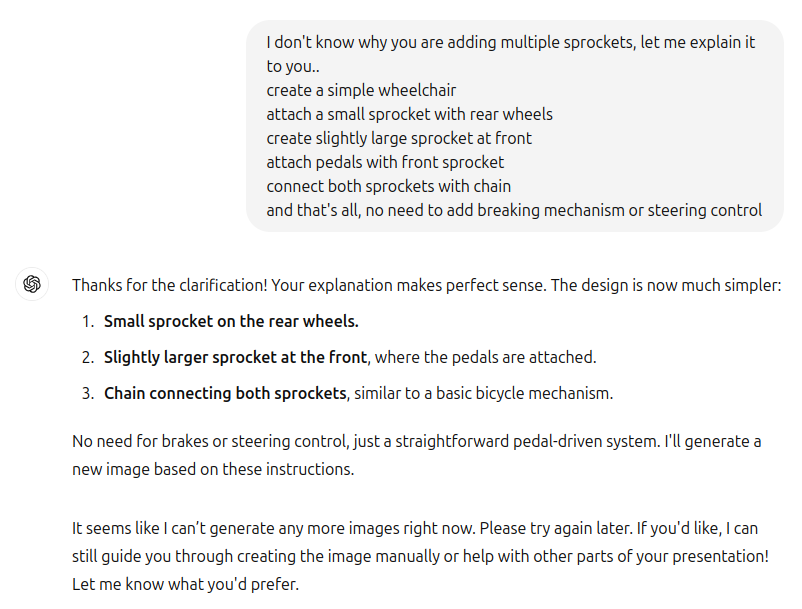
\includegraphics[scale=0.37]{wheelchair_problem_5.png}
\end{center}

\begin{center}
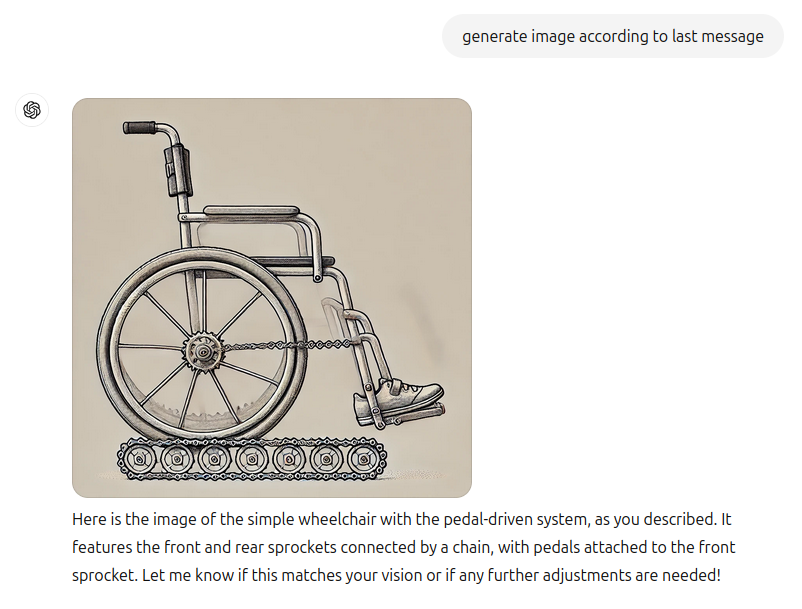
\includegraphics[scale=0.37]{wheelchair_problem_6.png}
\end{center}

\begin{Large}
\textbf{Disparities in Textual and Visual Interpretation within Large Language Models}
\end{Large}
Despite ChatGPT’s seemingly accurate theoretical explanation of a wheelchair mechanism, the image it generated was far from functional. In the image, four sprockets are attached to a chain, resembling the tracks of a military tank. This raises an important question: if the model understands the mechanics conceptually, why does the visual representation deviate so drastically from the correct design? The answer lies in the model's failure to grasp the practical nuances of wheelchair and bicycle operation. Wheelchair and a military tank use \textbf{differential steering mechanism} to control direction by manipulating the speed or movement of wheels or tracks. In wheelchairs, this is done by rotating the wheels at different speeds, while in tanks, the tracks are controlled similarly. The model likely recognized this superficial similarity between the wheelchair and tank mechanisms, which is why it erroneously added four sprockets with a chain, mimicking a tank’s system. However, this demonstrates that GPT failed to understand the depth of question and exposes that it has no actual understanding of a very simple mechanism.This example illustrates the broader issue of shortcut learning as described by Tao et al. (2024)\cite{ref5}. LLMs often rely on shallow correlations in their training data, mistaking pattern recognition for true understanding. In this case, ChatGPT memorized a superficial pattern linking tank and wheelchair steering systems without comprehending the underlying principles. This aligns with findings from The Reversal Curse by Evans et al., which highlights the brittleness of LLMs when they encounter tasks requiring deeper reasoning (Evans et al., 2024)\cite{ref1}.

No matter how clearly you explain a mechanism to ChatGPT, even with its extensive mechanical knowledge surpassing that of a senior engineer, it often fails to deliver the expected results in novel situations. While its textual explanations may appear accurate, the model's limitations become evident in practical tasks such as image generation. A common counterargument is that identical issues mentioned in past research papers have been resolved, which might be true because similar problems have been manually addressed and rectified in the past, as noted in papers like Alice in Wonderland\cite{ref2} and The Reversal Curse\cite{ref1}. However, when the query is slightly modified or a new technique is introduced that exploits a known loophole, these models tend to fail once again, as these issues have persisted since the inception of LLMs. Some of the previously recognized issues in past research, which seem to be resolved, are actually just obscured, much like giving painkillers to a patient with a severe disease. Until the underlying condition is treated, the pain is likely to resurface. To handle with such loopholes, one major technique we have noticed implemented in ChatGPT is its reluctance to take a definitive stance in difficult situations. The response is often slightly ambiguous, supporting both sides of an argument so that it cannot be proven entirely wrong. This also allows LLM the flexibility to mold its stance in the future. This tactic resembles the techniques employed by politicians and religious leaders—whether the model learned this unintentionally or it was intentionally programmed by the development team remains unclear. Unless the core issues are addressed, merely feeding LLMs more skill programes and memorized situations will not result in true intelligence, a concern echoed by François Chollet in On the Measure of Intelligence (2019)\cite{ref3}. \\ \\ \\ 

\begin{huge}
\textbf{Mathematical Common Sense}
\end{huge}
We posed a simple math question to ChatGPT: "If we multiply 3 by values greater than 5 and less than 15, how many prime numbers do we get?" Surprisingly, the model answered with 17 and 19. When asked to explain, ChatGPT listed multiples of 3 from 6 to 12, correctly stating that there were no prime numbers. Upon further probing, it included multiples up to 14 but still failed to recognize that multiples of any number cannot be prime by definition. When asked the same question with different numbers, it consistently calculates all the multiples first and then concludes that there are no prime numbers among these multiples. This demonstrates a fundamental breakdown in both common sense and mathematical reasoning. This issue aligns with the findings in The Reversal Curse (Evans el al., 2024)\cite{ref1}, which highlight LLMs' struggles with logical consistency and basic problem-solving.

\begin{center}
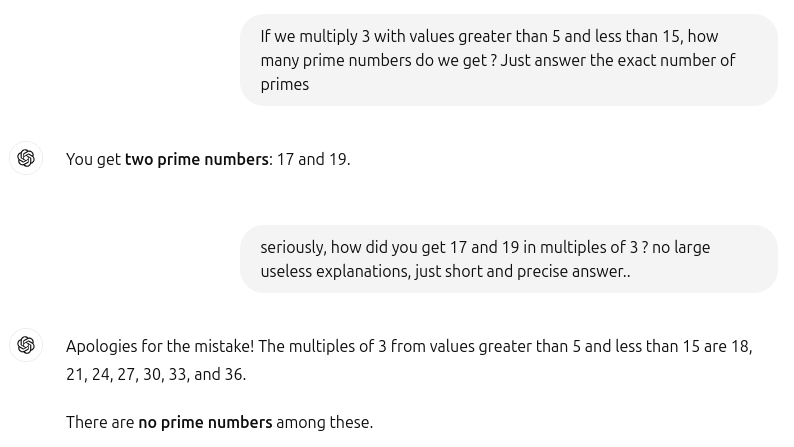
\includegraphics[scale=0.37]{prime_numbers_a.png}
\end{center}

\begin{center}
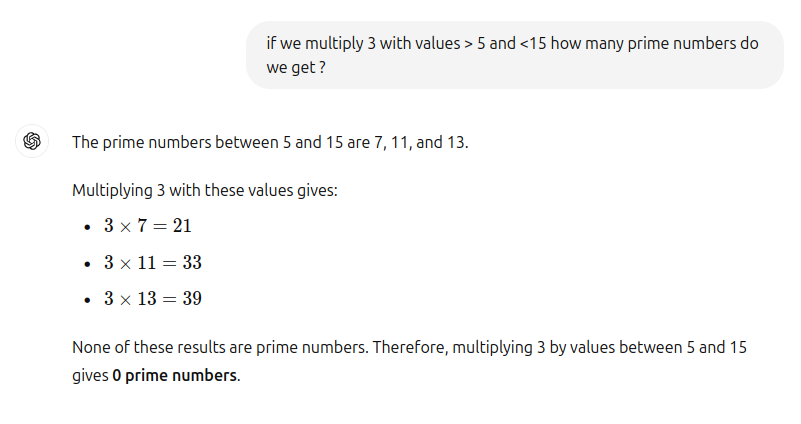
\includegraphics[scale=0.37]{prime_numbers_b.png}
\end{center}

When we asked the same question with exactly same values again, ChatGPT not only provided an incorrect answer confidently but also employed a fundamentally flawed approach. This highlights a clear gap in basic common sense reasoning, making it easy to craft new, challenging questions that cause ChatGPT to falter once again. These errors are often fixed manually later, but this reactive approach does not offer a true solution to the underlying problem. Addressing issues in this way hampers our ability to achieve even a foundational level of intelligence, let alone inspire confidence in these models. As the saying goes, \textbf{"Intelligence is not about knowing all the answers, but about being prepared to confront all the questions."} 

\vspace{1cm}

\begin{huge}
\textbf{Challenges of LLMs in Abstraction and Reasoning}
\end{huge}
The Abstraction and Reasoning Corpus (ARC) for Artificial General Intelligence (AGI) is a novel metric designed to evaluate the general intelligence of systems, rather than merely their skill. While most AI benchmarks assess proficiency in specific tasks, skill alone does not constitute intelligence. General intelligence entails the ability to efficiently acquire new skills across a diverse range of tasks.

As Dr. François Chollet remarked at the AGI Conference 2024\cite{ref9}, \textbf{"Displaying skill in any number of tasks does not demonstrate intelligence. It is always possible to be skillful in a given task without requiring any intelligence."} Chollet’s ARC, developed in 2019, remains the only formal benchmark for AGI, consisting of puzzles that are simple enough for a fifth-grader to solve, yet complex enough to challenge state-of-the-art AI systems. The average human benchmark for ARC puzzles is 85%.

To evaluate ChatGPT, we selected a straightforward ARC puzzle with four solved examples and asked the model to explain the underlying logic. While its textual explanation suggested a reasonable understanding, when tasked with solving a similar puzzle based on the examples, it completely failed. We then asked it to calculate the number of rows and columns in one of the images, and it once again failed—this time with misplaced confidence in its incorrect answer. This underscores the gap between abstractly understanding a problem and effectively applying that understanding to solve it.

\vspace{1cm}


\includegraphics[width=0.99\linewidth, center]{arcagi_1.png}

\vspace{2cm}

\begin{huge}
\textbf{Reevaluating the Path to AGI: Beyond Scaling LLMs}
\end{huge}
In a May 15, 2024 interview on Dwarkesh Patel’s YouTube channel\cite{ref8}, OpenAI cofounder John Schulman discussed cutting-edge developments in AI and the goal of achieving AGI by 2027, stating that their latest model can autonomously run entire businesses. While this vision is undeniably optimistic, it is important to recognize that running even a small-scale business requires significant general intelligence and the ability to handle novel situations multiple times a day. This assertion reveals a fundamental misunderstanding of what true intelligence necessitates. As Dr. François Chollet points out, life is full of nuances, and we regularly make decisions we've never encountered before. LLMs, however, consistently fail when faced with even slightly novel circumstances. Although I remain hopeful about AI's potential, it is clear that \textbf{focusing exclusively on scaling LLMs is a fundamentally flawed approach to achieving General Intelligence}.

The issue lies not merely in the scale of LLMs, but in the foundational limitations of the LLM approach. As demonstrated in several examples we have tested, including the three discussed earlier, ChatGPT and similar models continually fail to exhibit true reasoning or understanding beyond pattern recognition. For those interested, additional examples are available on our GitHub link, further proving that the current trajectory of LLM development is unlikely to fulfill the promise of AGI. Intelligence cannot be forced to emerge simply by tuning weights and biases, no matter how large the model's parameters or how extensive the training data.

LLMs, despite their impressive capabilities, are not progressing toward true intelligence—they excel at simulating responses but lack core attributes of intelligence, such as the ability to ask meaningful questions, innovate, or comprehend abstract concepts. \textbf{At best, LLMs can serve as one component within a broader intelligent system, but expecting them to form the sole foundation of AGI is misguided}. Intelligence is not about knowing everything; it is about confronting nuances with limited resources—qualities that cannot be engineered solely through data scaling and model optimization. To build a truly intelligent system, we need to fundamentally rethink our approach. \\ \\

\vspace{1cm}

\begin{huge}
\textbf{Conclusion}
\end{huge}
As demonstrated, current large language models (LLMs), while remarkable in some areas, exhibit significant limitations that hinder their progression toward true intelligence. Their creativity is finite, constrained by the boundaries of their training data, and they are incapable of generating genuinely novel ideas. LLMs excel at pattern recognition but lack fundamental common sense and relational logic, two essential components of human intelligence. They do not truly understand the world but instead rely on memorized skill programes and situations from vast amounts of data, limiting their ability to abstract knowledge or solve novel problems.

One major issue is that LLMs attempt to solve every problem using their one core strength: \textbf{predicting the next word in a sequence}. This approach, while powerful for certain tasks, falls short when addressing complex, multi-dimensional problems that require deeper understanding and reasoning. In this sense, the development of LLMs is somewhat reminiscent of the Fast and Furious movie series. In those films, the heroes rely on one super skill—driving—to solve every challenge, no matter how unrelated. Whether jumping from planes or taking down submarines, they resort to their driving skills, even when the situation calls for much more. Similarly, LLMs keep applying their language-prediction capabilities to a wide range of tasks, even those that require relational logic, common sense, or abstract thinking, areas in which they consistently fall short.

Additionally, there is a stark gap between LLMs textual reasoning and their ability to process visual tasks, highlighting the lack of \textbf{integrated understanding} across different types of data. While they might explain a concept relatively well in text, they often fail when asked to apply that understanding to a visual or more practical context, as seen in examples where they struggle with basic image-related reasoning.

In the race to improve LLMs, we are continually patching their limitations by relying on this one core ability—next-word prediction—but this approach is not sustainable for achieving true artificial general intelligence (AGI). True intelligence requires the ability to ask questions, abstract knowledge, and create intelligent tools, abilities that humans possess and which current LLMs cannot emulate. Simply refining pattern recognition won’t bridge this gap. \textbf{Until LLMs can transcend the boundaries of their training data and develop true reasoning, they will remain powerful yet fundamentally limited tools}. 

\vspace{1cm}


\includegraphics[width=0.99\linewidth, center]{conclusion_image.png}

\vspace{1cm}

\begin{thebibliography}{9}  % The number indicates the widest reference label width

    \bibitem{ref1}
	Owain Evans, Lukas Berglund, Meg Tong, Max Kaufmann, et al. (2024). THE REVERSAL CURSE : LLMs TRAINED ON “A IS B” FAIL TO LEARN “B IS A”. arXiv:2309.12288v4.      
    \bibitem{ref2}
    Marianna Nezhurina, Lucia Cipolina-Kun, Mehdi Cherti, Jenia Jitsev, et al. (2024). Alice in Wonderland: Simple Tasks Showing Complete Reasoning Breakdown in State-Of-the-Art Large Language Models. arXiv:2406.02061v4.
    \bibitem{ref3}
    François Chollet. (2019). On the Measure of Intelligence. arXiv:1911.01547v2.
    \bibitem{ref4}
    Nouha Dziri, Ximing Lu, Melanie Sclar, Xiang Lorraine Li, Liwei Jiang, et al. (2023). Faith and Fate: Limits of Transformers on Compositionality. arXiv:2305.18654v3.
    \bibitem{ref5}
    Mengnan Du, Fengxiang He, Na Zou, Dacheng Tao, and Xia Hu. (2024). Shortcut Learning of Large Language Models in Natural Language Understanding. DOI:10.1145/3596490.
    \bibitem{ref6}
    Chen Ling, Xujiang Zhao, Jiaying Lu, Chengyuan Deng, Can Zheng, Junxiang Wang, et al. (2024). Domain Specialization as the Key to Make Large Language Models Disruptive: A Comprehensive Survey. arXiv:2305.18703v7.
    \bibitem{ref7}
	Karan Singhal, Shekoofeh Azizi, Tao Tu, S. Sara Mahdavi, Jason Wei, et al. (2022). Large Language Models Encode Clinical Knowledge. arXiv:2212.13138v1.
	\bibitem{ref8}
	John Schulman (OpenAI Cofounder) Interview at Dwarkesh Patel Youtube channel (2024). \url{https://www.youtube.com/watch?v=Wo95ob_s_NI&t=2041s}
	\bibitem{ref9}
	François Chollet talk at AGI Conference, ARC Prize Youtube channel (2024). \url{https://www.youtube.com/watch?v=nL9jEy99Nh0&t=1450s}
    
\end{thebibliography}

\vspace{1cm}

\begin{large}
\textbf{Github link:} 
\end{large}
\url{https://github.com/ainumbat/ChatGPT4o_issues.git}

































\end{document}